\documentclass[]{article}
\usepackage{amsmath}
\usepackage{amsthm}
\usepackage{listings}
\usepackage{graphicx}
\usepackage{hyperref}
\usepackage{cleveref} %for the cref command

\title{Practical Lab Numerical Computing Computational Finance \\Bachelor-Worksheet 3}
\author{Lukas Troska, Ilja Kalmykov}
\date{}
\setlength{\parindent}{0pt}

\begin{document}

\maketitle

The referenced source code files can be found on
\url{https://github.com/iljaGH/CompFin/}.

\section*{Task 2}
See task2.cpp for code.

\section*{Task 3}
As we can see \Cref{fig:Task3a,fig:Task3b}, the number of time steps does not
affect the convergence at all.
\begin{figure}[!ht]
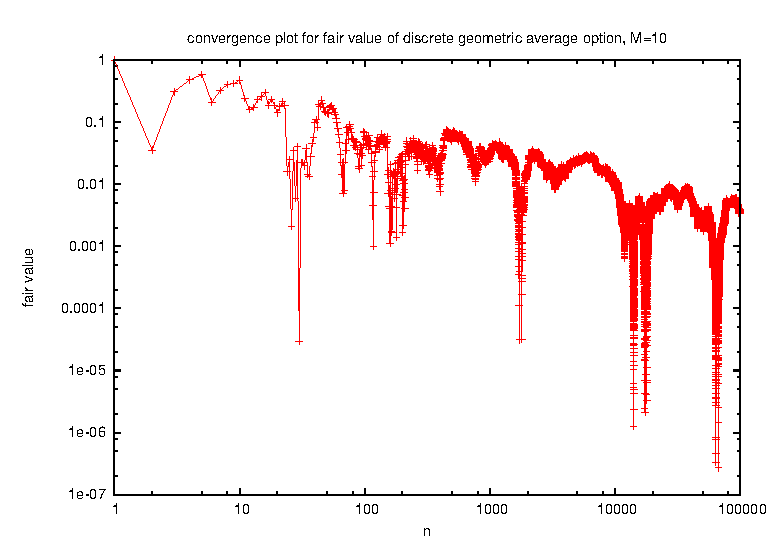
\includegraphics[width=.9\textwidth]{task3_10.eps}
\caption{Convergence plot for the fair value of diskrete geometric average
option, $M = 10$.}
\label{fig:Task3a}
\end{figure}
\begin{figure}[!ht]
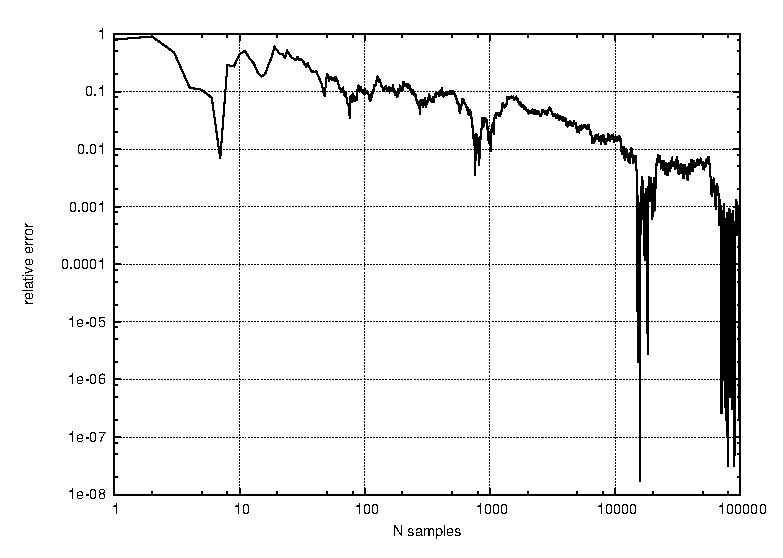
\includegraphics[width=.9\textwidth]{task3_200.eps}\\
\caption{Convergence plot for the fair value of diskrete geometric average
option, $M = 200$.}
\label{fig:Task3b}
\end{figure}
\clearpage

\section*{Task 4} See task4.cpp for code and \Cref{fig:Task4}. The convergence
is $N^{-0.5}$. The last increase in error is because of the limitations of
the datatype int. For $M\ge 1024$ we get under-/overflows in our calculation
because the numbers are too big.
\begin{figure}[!ht]
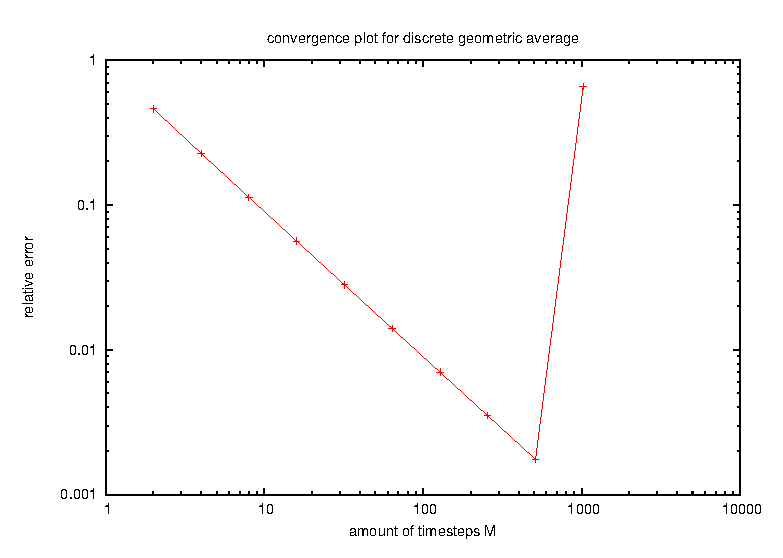
\includegraphics[width=.9\textwidth]{task4.eps}
\caption{Convergence plot for the diskrete geometric average.}
\label{fig:Task4}
\end{figure}
\clearpage

\section*{Task 5} See task5.cpp for code and \Cref{fig:Task5a,fig:Task5b}). The
integrand of the discrete arithmetic average for $M=2$ looks like:
\begin{figure}[!ht]
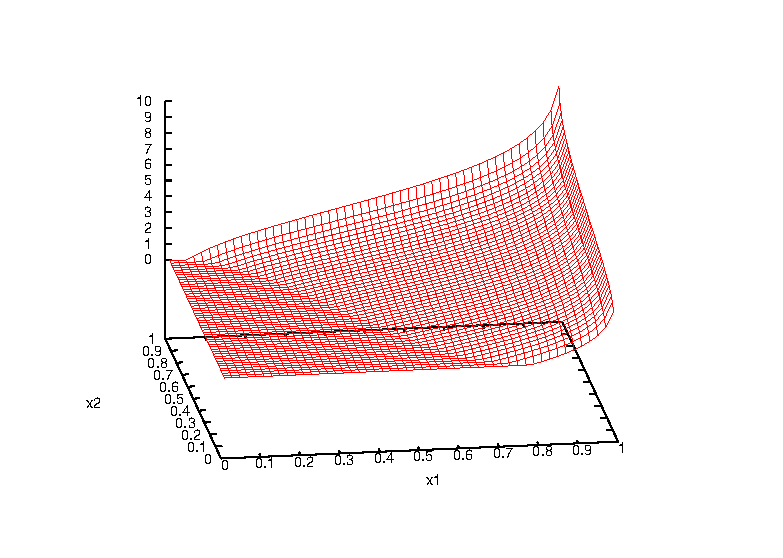
\includegraphics[width=.9\textwidth]{task5_1}
\caption{Integrand for discrete arithmetic average, $M=2, S(0)=10, r=0.1,
\sigma=0.25, T=1, K=10$.}
\label{fig:Task5a}
\end{figure}
\begin{figure}[!ht]
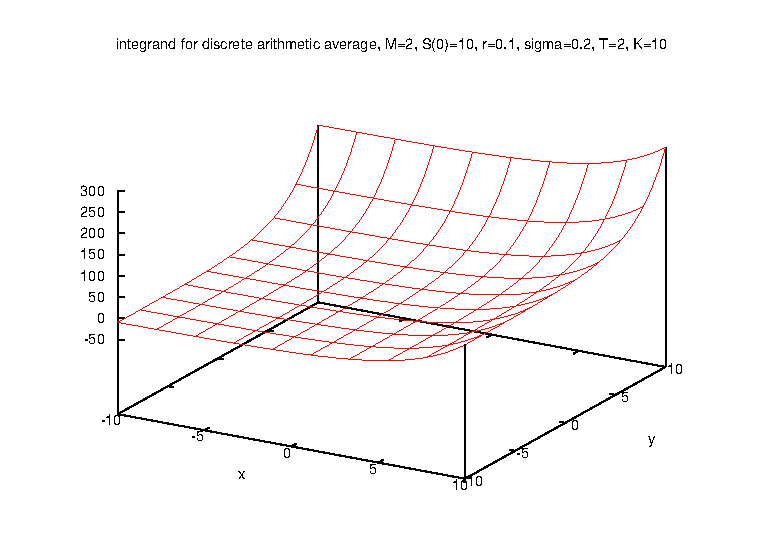
\includegraphics[width=.9\textwidth]{task5_2}
\caption{Integrand for discrete arithmetic average, $M=2, S(0)=10, r=0.1,
\sigma=0.2, T=2, K=10$.}
\label{fig:Task5b}
\end{figure}
\clearpage


\section*{Task 6}
See task6.cpp for code.

\section*{Task 7} See task7.cpp for code. In \Cref{fig:task_7a} is a plot of the
first 100 members of the Halton sequence for $d=2$ and 100 uniform random numbers on
$(0,1)^2$ in \Cref{fig:task_7b}. As we can see, the Halton sequence covers the
unit square more evenly than uniformly distributed points, i.e. "gaps" between the points are not as
big.
\begin{figure}[!ht]
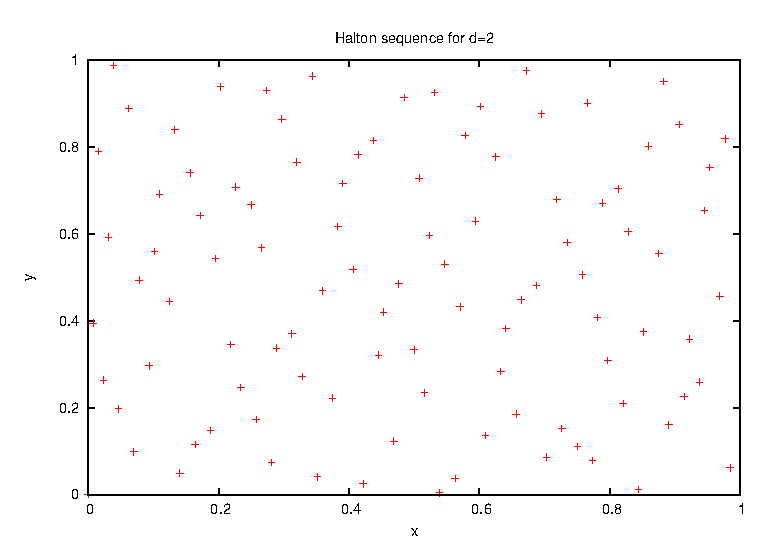
\includegraphics[width=.9\textwidth]{task7_halton.eps}
\caption{Halton sequence for $d=2$.}
\label{fig:Task7a}
\end{figure}
\begin{figure}[!ht]
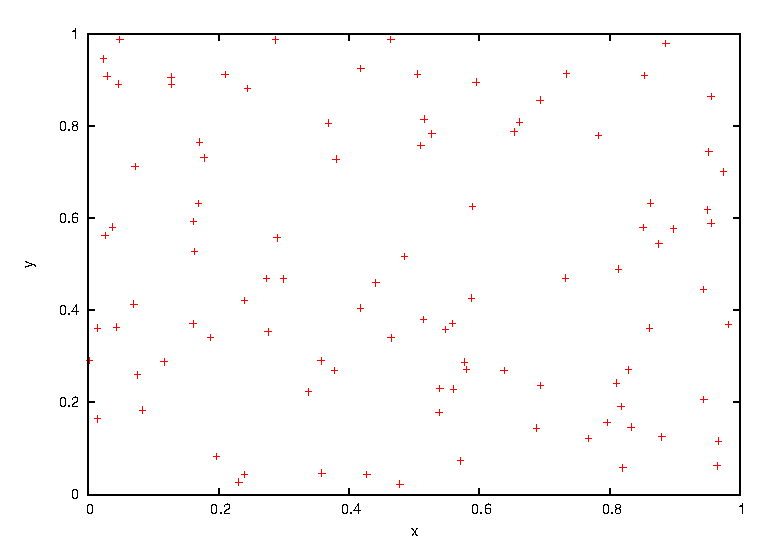
\includegraphics[width=.9\textwidth]{task7_uniform.eps}
\caption{Uniform random numbers on unit square.}
\label{fig:Task7b}
\end{figure}
\clearpage


\section*{Task 8}
See task8.cpp for code.

\section*{Task 9}
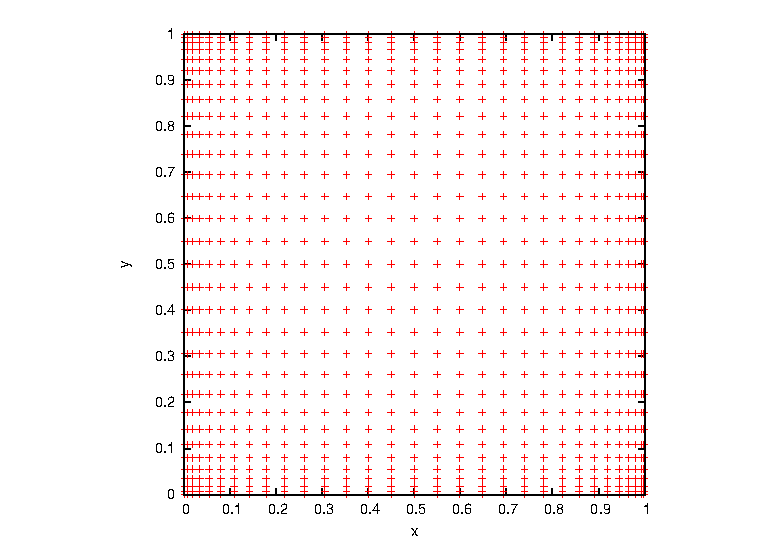
\includegraphics[width=.9\textwidth]{task9_gauss}\\
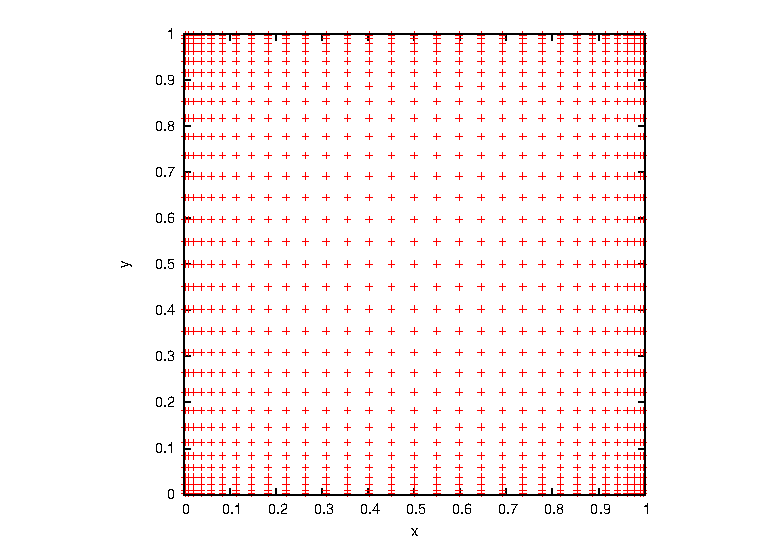
\includegraphics[width=.9\textwidth]{task9_cc}\\
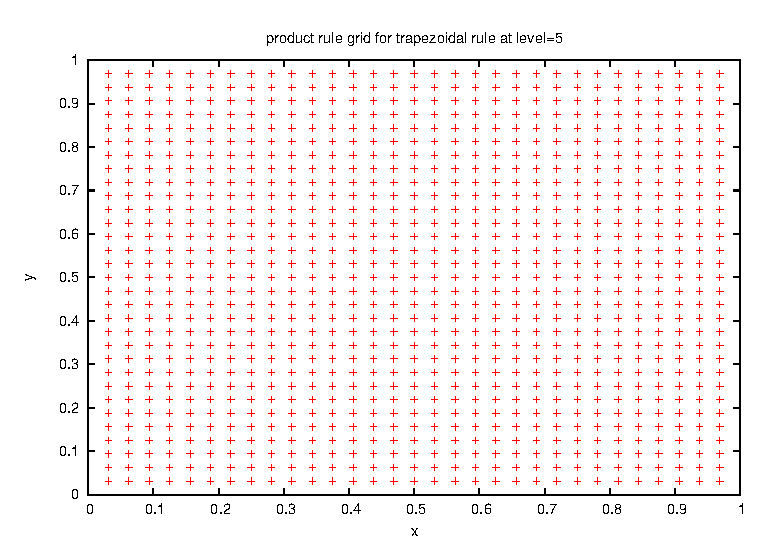
\includegraphics[width=.9\textwidth]{task9_trapezoidal}\\

\section*{Task 10}
See task10.cpp for code.

\section*{Task 11}
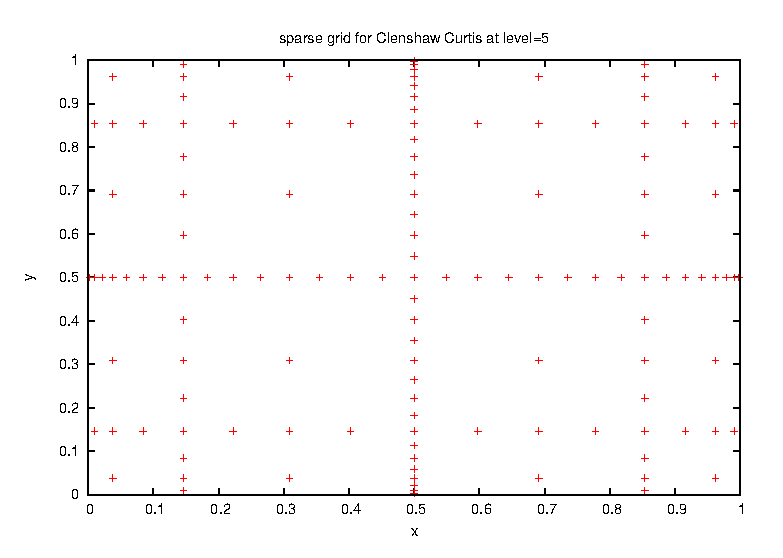
\includegraphics[width=.9\textwidth]{task11_cc5}\\
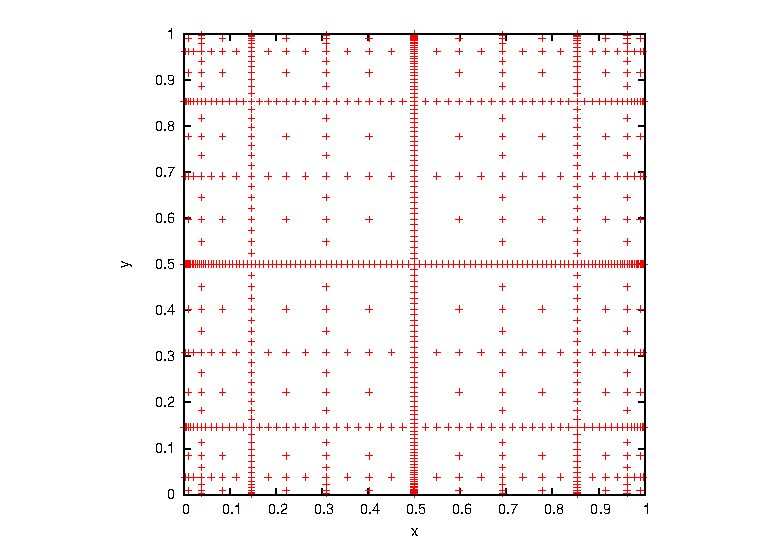
\includegraphics[width=.9\textwidth]{task11_cc7}\\
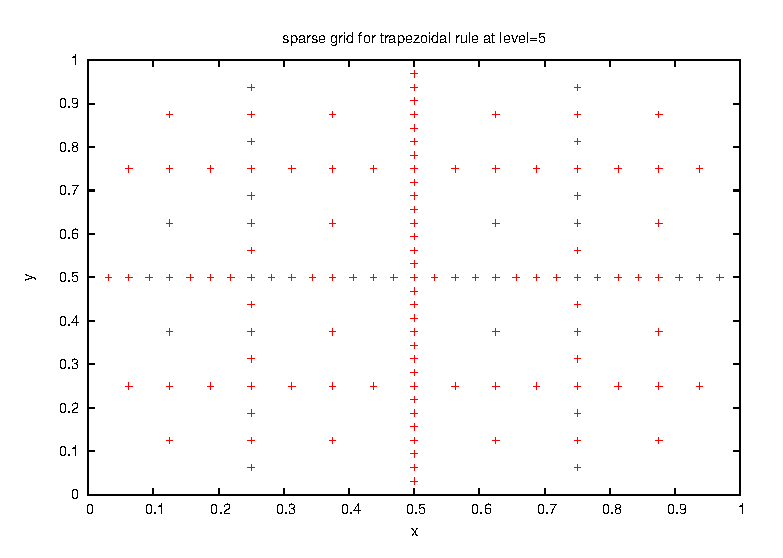
\includegraphics[width=.9\textwidth]{task11_trap_5}\\
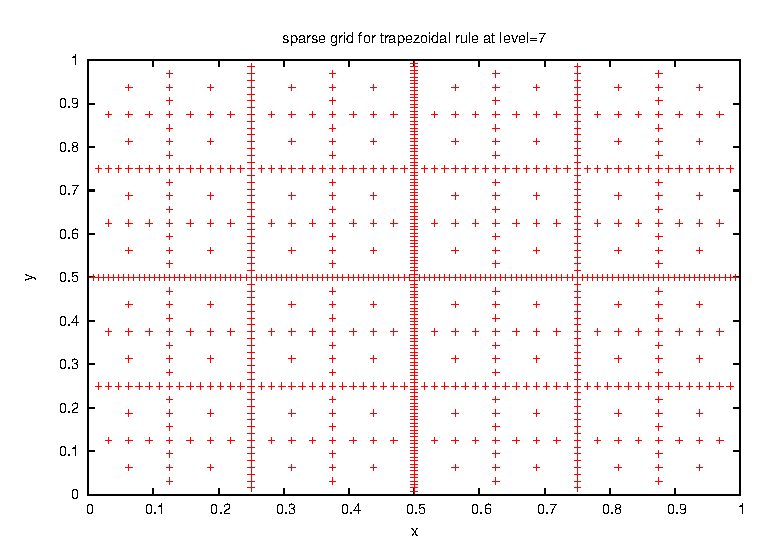
\includegraphics[width=.9\textwidth]{task11_trap_7}\\

\section*{Task 12}
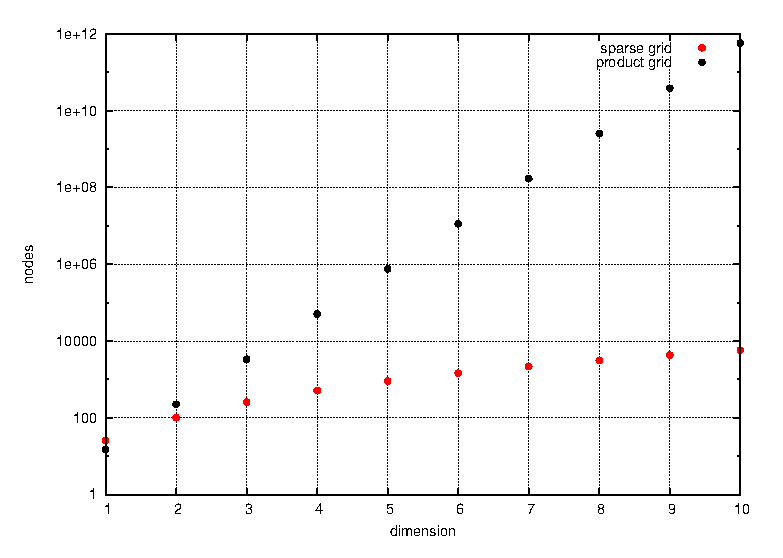
\includegraphics[width=.9\textwidth]{task12}\\

\section*{Task 13}
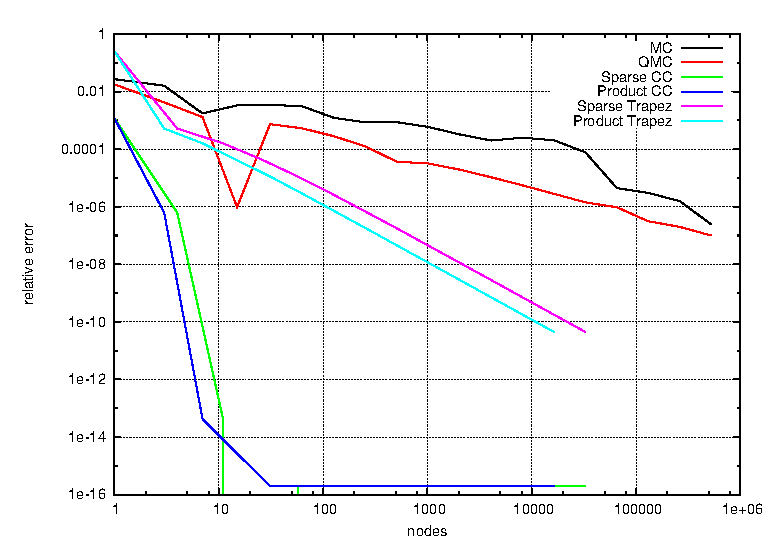
\includegraphics[width=.9\textwidth]{task13_d1}\\
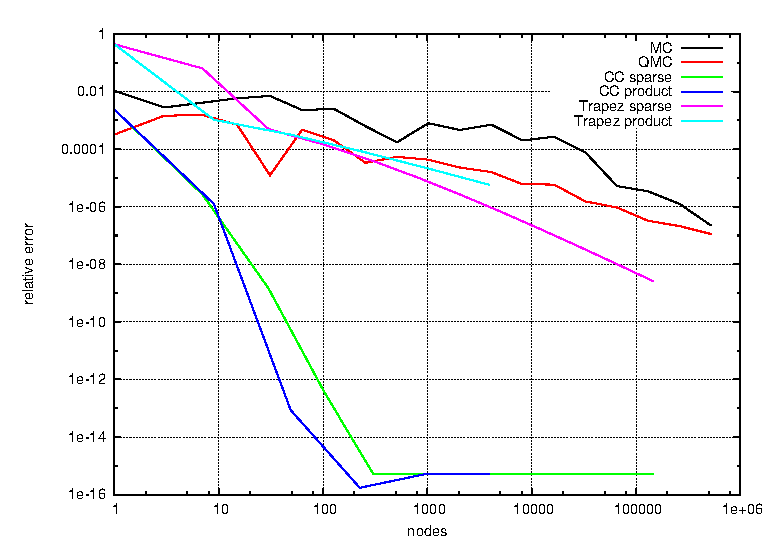
\includegraphics[width=.9\textwidth]{task13_d2}\\
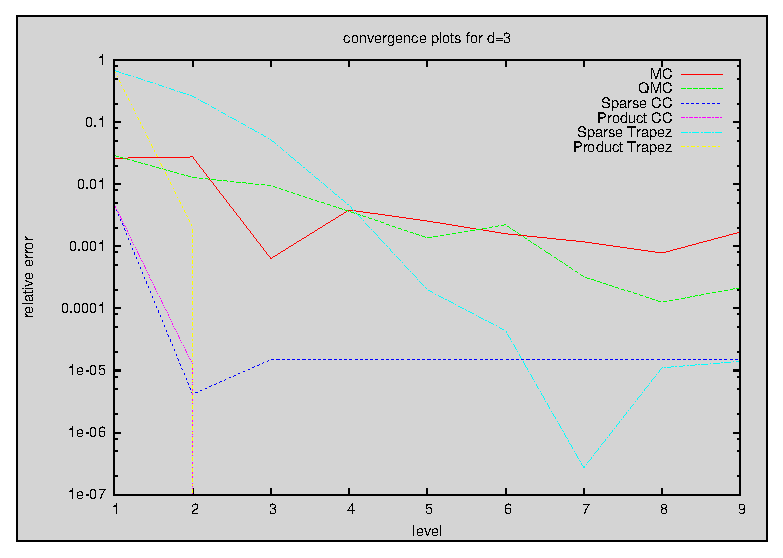
\includegraphics[width=.9\textwidth]{task13_d4}\\
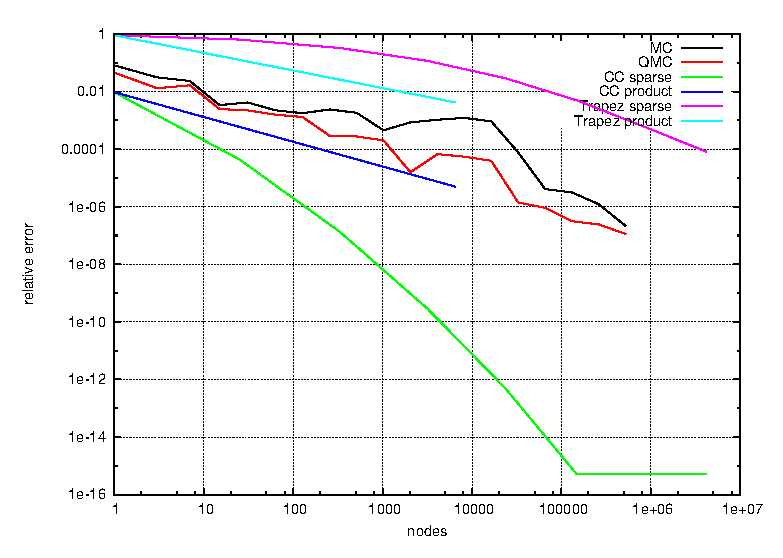
\includegraphics[width=.9\textwidth]{task13_d8}\\

\section*{Task 14}
See task14.cpp/task15.cpp

\section*{Task 15}
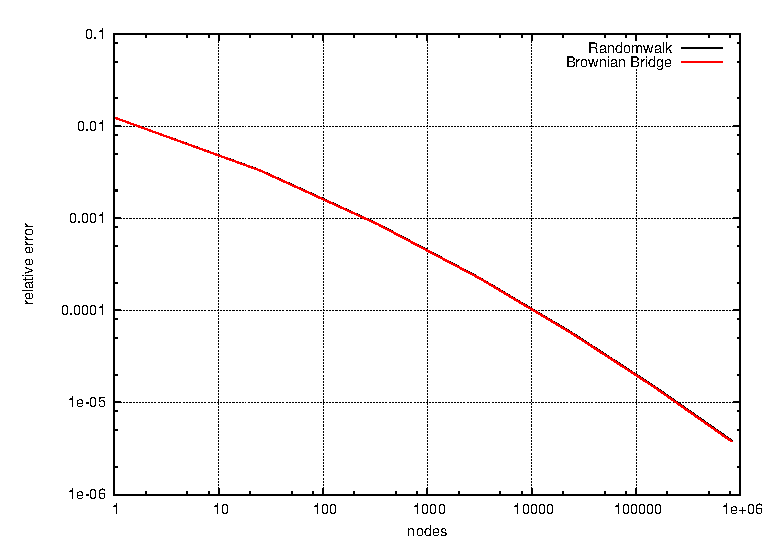
\includegraphics{task15}\\

\section*{Task 16}
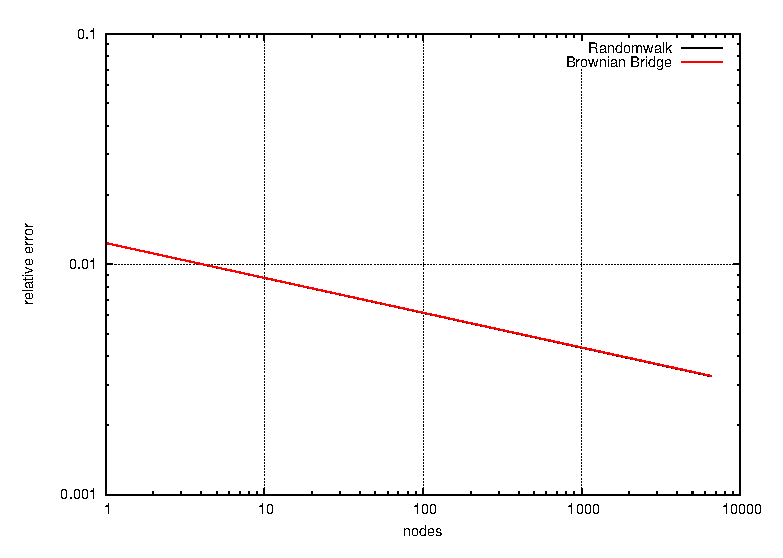
\includegraphics{task16_ccprod}\\
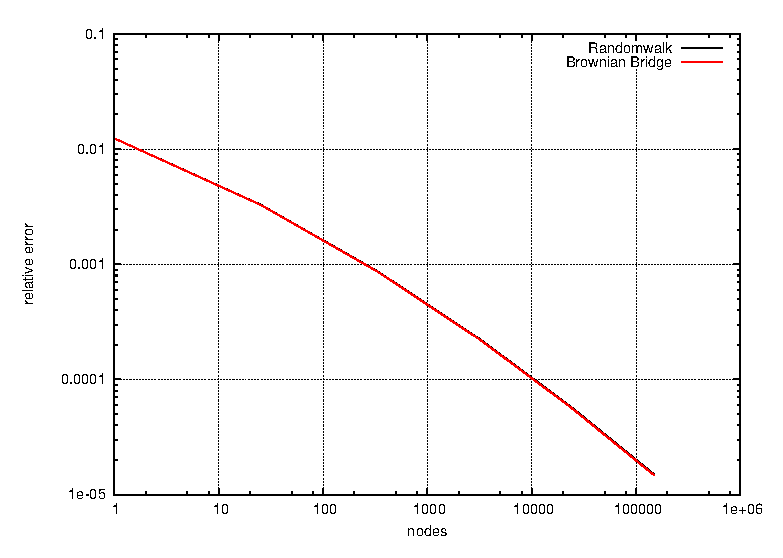
\includegraphics{task16_ccsparse}\\
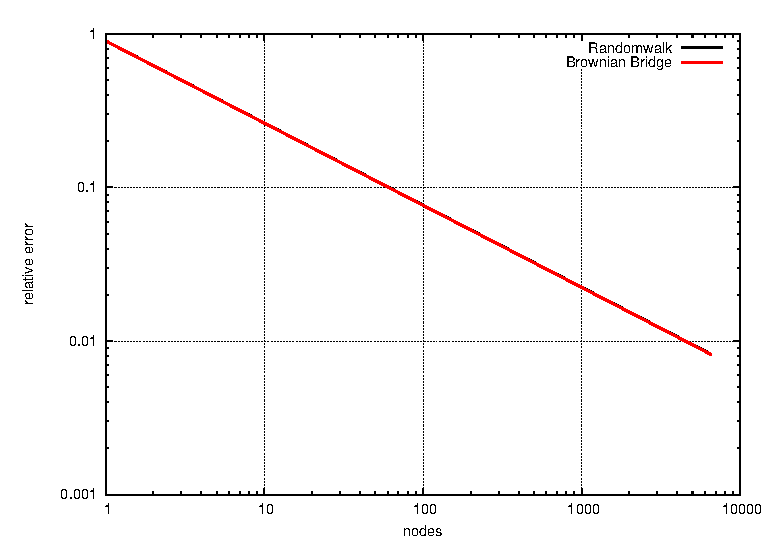
\includegraphics{task16_trapprod}\\
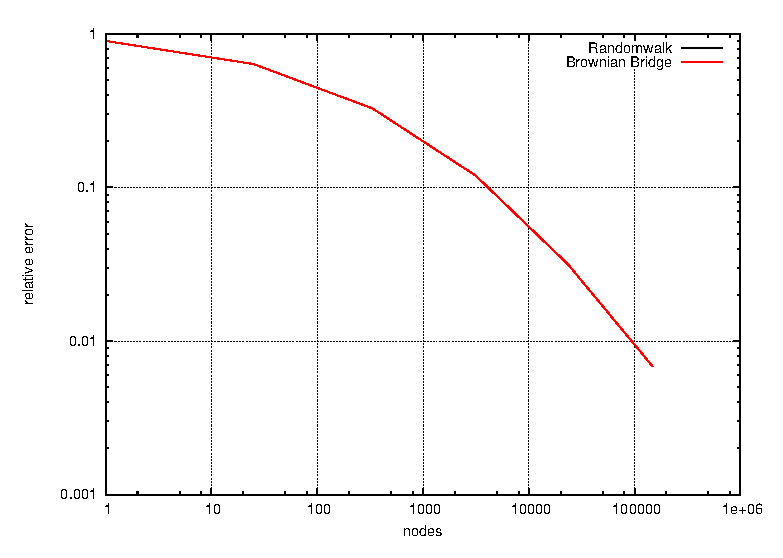
\includegraphics{task16_trapsparse}\\
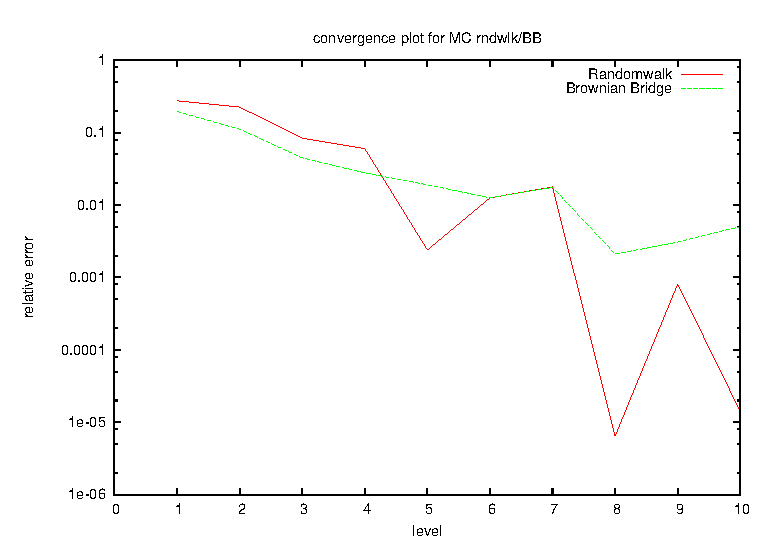
\includegraphics{task16_mc}\\
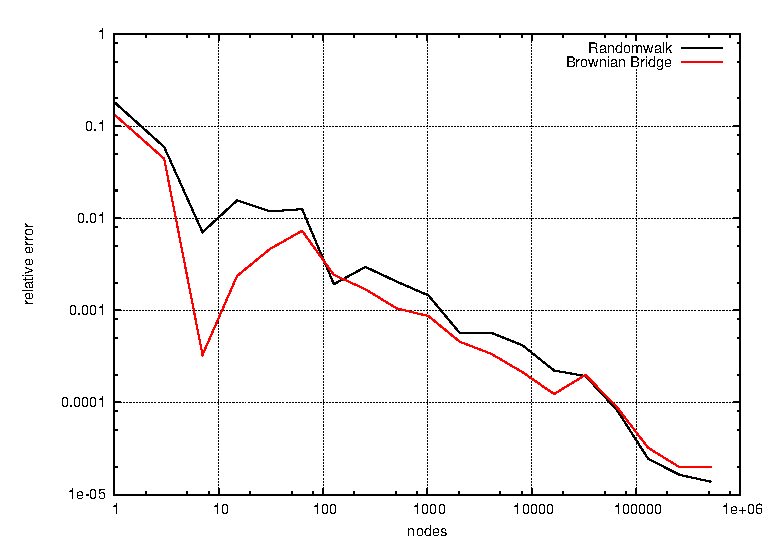
\includegraphics{task16_qmc}\\

\section*{Task 17}
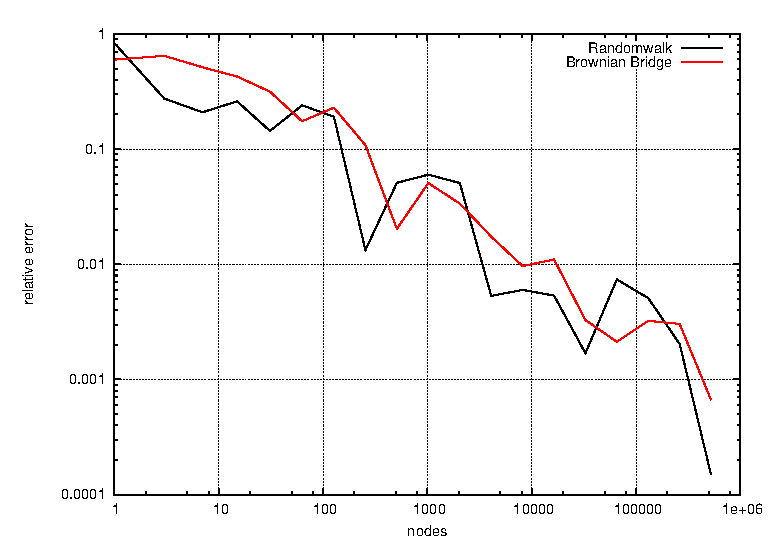
\includegraphics{task17_mc}\\
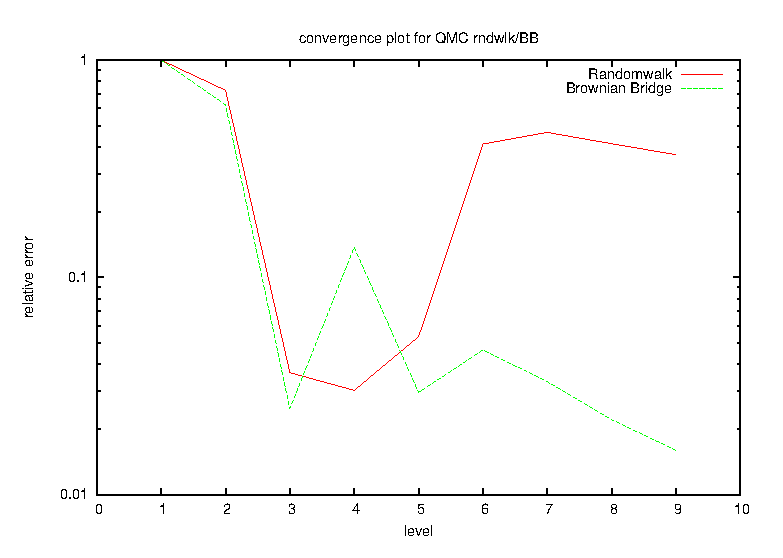
\includegraphics{task17_qmc}\\

\section*{Task 18} It is almost always better to not use (Q)MC, since the other
quadrature rules converge faster (even using full grids). Clenshaw-Curtis
converges slightly faster than the Trapezoidal rule. In almost all cases sparse
grids are preferrable Since they only give us a slightly worse convergences, but
way less points of evaluation (see Task 12). But if everything else fails, (Q)MC
works (but might converge slowly).
\end{document}
